\chapter{Caso práctico}\label{cap:09caso}
En este capítulo se divide en cinco secciones: \ref{sec:09intro} Introducción, \ref{sec:09huvr} Estudio realizado por el HUVR, \ref{sec:09atlas} Estandarización del estudio con ATLAS, \ref{sec:09resultados} Discusión de resultados y \ref{sec:09conclusiones} Conclusiones.

\section{Introducción} \label{sec:09intro}

Este capítulo pretende demostrar la relevancia de OHDSI (Observational Health Data Science and Informatics) y la utilidad de sus herramientas, concretamente el uso de ATLAS para la estandarización y reproducibilidad de los análisis clínicos observacionales sobre bases de datos estandarizadas al Modelo de Datos Común de OMOP. 

Para ello, bajo la tutela de D. Carlos Parra y Da. Silvia Rodríguez (tutores de las prácticas en empresa, véase \ref{sec:03Participantes} ''Participantes del proyecto''), se ha seguido la reproducción de un estudio realizado por investigadores del hospital sobre predicción mediante modelos de ML de efectos adversos en el tratamiento radioterápico de pacientes con cáncer de pulmón. 

Este estudio, se encuentra públicamente accesible en Pubmed en dos artículos, el primero publicado en el año 2019 titulado \textit{''Comparison of Feature Selection Methods for Predicting RT-Induced Toxicity'' }\cite{nunez2019comparison} y el segundo, en 2023 titulado \textbf{\textit{''Benchmarking machine learning approaches to predict radiation-induced toxicities in lung cancer patients''}} \cite{nunez2023benchmarking}. Ambos estudios están también publicados en la ruta \code{Thesis-ATLAS-OHDSI/documentation/pdf/estudioHUVR} del repositorio de github del TFG \cite{vallealonsodc}.

El objetivo es promover el uso de ATLAS para la investigación observacional, reproduciendo mediante ATLAS un estudio que fue realizado sin hacer uso de la herramienta, para demostrar con un caso práctico los beneficios de utilizar la herramienta en términos de reproducibilidad y estandarización.

\section{Estudio realizado por el HUVR} \label{sec:09huvr}

El estudio consiste en la comparación de 300 modelos de ML sobre un dataset de 875 pacientes de cancer de pulmón con el objetivo de predecir los efectos adversos a corto (esofagitis, tos, disnea y neumonitis) y a largo plazo (disnea y neumonitis) que producirá el tratamiento radioterápico sobre estos pacientes. 

\subsubsection{Contexto}

%La base teórica del estudio \cite{nunez2019comparison, nunez2023benchmarking} es que la radioterapia aunque es beneficiosa para el tratamiento oncológico, también causa efectos perjudiciales a corto y/o  largo plazo de forma personalizada según las condiciones de cada paciente. El auge de la medicina personalizada y centrada en el paciente (véase \ref{sec:01Contexto}) ha ensalzado la importancia de realizar una planificación individual para cada paciente, pues cada persona responde de forma distinta a los tratamientos. Por tanto, la gestión individualizada de los posibles efectos adversos es muy importante en la planificación del tratamiento radioterápico, con el fin de facilitar la toma de decisiones entre médico y paciente en términos de calidad de vida y posibilidades de supervivencia.

La radioterapia, aunque beneficia el tratamiento oncológico, puede ocasionar efectos perjudiciales a corto y largo plazo, de forma personalizada según cada paciente \cite{nunez2019comparison, nunez2023benchmarking}. La medicina centrada en el paciente (véase \ref{sec:01Contexto} ''Marco contextual'') destaca la importancia de planificar individualmente cada tratamiento, dado que las respuestas varían entre individuos. Por tanto, la gestión personalizada de los efectos adversos es crucial en la planificación radioterápica para facilitar la toma de decisiones médico-paciente en términos de calidad de vida y supervivencia.

\subsubsection{Objetivo}

El objetivo del estudio es utilizar un conjunto de datos del mundo real (RWD) para facilitar la toma de decisiones clínicas, estudiando para cada efecto adverso del tratamiento radioterápico, el modelo de ML que provee una mejor predicción en términos de precisión del modelo (AUC).

\subsubsection{Datos}

- RWHD

\textcolor{red}{- 875 pacientes del registro s31 y observacion del huvr??}

\subsubsection{Metodología}

Para conformar los 300 modelos de ML se han entrenado y testeado 5 modelos de ML combinados con 10 métodos de selección de atributos (\textit{Feature Selection, FS}) sobre 6 efectos adversos (\textit{outcomes} o \textit{clinical endpoints}), de la siguiente forma: 

\begin{itemize}
    \item \textbf{5 Modelos de ML}. Se utilizaron cinco clasificadores basados en aprendizaje 
    automático: 
    \begin{itemize}[label={--}]
        \item Máquina de Vectores de Soporte (\textit{Support Vector Machine, SVM}).
        \item Vecinos más Cercanos (\textit{k-Nearest Neighborhood, kNN}).
        \item Red Neuronal Artificial (\textit{Artificial, Neural Network, ANN}) de alimentación directa.
        \item Modelo Lineal Generalizado (\textit{Generalized Linear Model, GLM}).
        \item Clasificador de Naïve-Bayes (\textit{NB}).
    \end{itemize}
     Los hiperparámetros de los modelos se se optimizaron automáticamente siguiendo ''las recomendaciones de la literatura''.
    
    \item \textbf{10 Métodos de Selección de Atributos \textit{(FS)}.} Para reducir la dimensionalidad de los conjuntos de datos, se implementaron los siguientes métodos:
    
    \begin{itemize}[label={--}]
        \item Selección de Características Basada en Correlación (\textit{Correlation-based Feature Selection, CFS}).
        \item Chi-cuadrado %(\( \chi^2 \)).
        \item Boruta.
        \item Mínima Redundancia - Máxima Relevancia (\textit{Minimum Redundancy-Maximum Relevance, mRMR}).
        \item Relief.
        \item Ganancia de Información (\textit{Information Gain, IG}).
        \item  Bosque Aleatorio (\textit{Random Forest, RF}).
        \item 2 métodos de ensamblaje a partir de métodos de FS individuales y de subconjuntos.
        \item Subconjuntos de variables determinadas por un oncólogo experto para predecir las toxicidades seleccionadas basadas en la evidencia clínica.
    \end{itemize}

    \item \textbf{6 Efectos adversos.} Se seleccionaron seis efectos adveros a estudiar, clasificados según si su duración fue a corto plazo y a largo plazo. A corto plazo:
    \begin{itemize}[label={--}]
        \item Esofagitis.
        \item Tos.
        \item Disnea. 
        \item Neumonitis. 
    \end{itemize}
    A largo plazo:
    \begin{itemize}[label={--}]
        \item Disnea. 
        \item Neumonitis. 
    \end{itemize}
    Se consideran efectos adversos crónicos o a largo plazo si los efectos se mantuvieron presente más de tres meses a partir del inicio del tratamiento.
\end{itemize}

Para la validación interna de los modelos se ha utilizado una estrategia de validación cruzada de 10 pliegues (\textit{10-fold Cross-Validation}) en la que se aplicó una técnica de submuestreo aleatorio para generar un conjunto de datos equilibrado. Para la validación externa, se han utilizado los datos generados con los casos registrados después del 31 de mayo de 2018, que no fueron utilizados para la validación interna. 

Por último, el rendimiento de los modelos se ha medido en términos del AUC logrado por cada modelo predictivo.

\subsubsection{Resultados}

   Los resultados del estudio resaltan para cada outcome el mejor modelo de ML y selección de atributos, con la valoración de AUC en validación interna y externa. Los resultados se muestran de forma muy intuitiva en la siguiente tabla, extraída del artículo del HUVR \cite{nunez2023benchmarking}.

\begin{figure}[H]
    \centering
    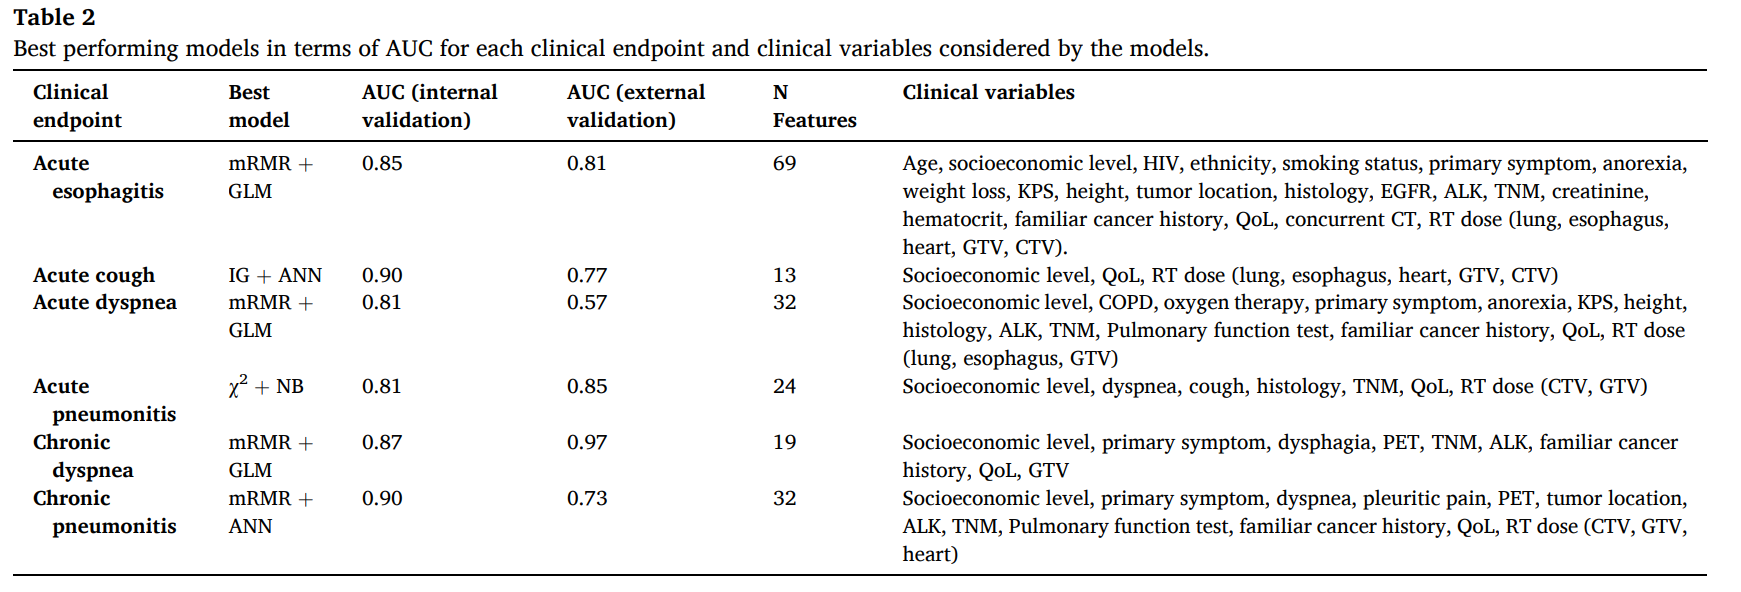
\includegraphics[width=1\textwidth]{tables/nune2023table2.png}
    \captionof{table}{Recopilación de resultados del estudio del HUVR. Extraída de \cite{nunez2023benchmarking}}
    \label{table:nune2023table2}
\end{figure}


\section{Estandarización del estudio con ATLAS} \label{sec:09atlas}

Este capítulo presenta finalmente el caso práctico realizado por la alumna en el que se aplican todos los contenidos teóricos y herramientas presentadas a lo largo de la memoria para realizar un análisis de datos real.

%\subsubsection{Objetivo}

\textbf{El objetivo de este estudio se alinea con el objetivo de OHDSI: estandarizar la investigación clínica observacional}, en este caso mediante el Modelo de Datos Común de OMOP y la herramienta de análisis de datos ATLAS. Es decir, no se pretende meramente reproducir el estudio haciendo uso del ecosistema de OHDSI sino que se destaca que el fin último del proceso es estandarizarlo, adaptarlo al marco de investigación OHDSI para que cualquier nodo de la organización pudiera procesarlo, analizarlo y reproducirlo fácilmente. 

%\subsubsection{Ádaptación del estudio al marco de OHDSI}

\textbf{El estudio realizado por el HUVR en el marco de OHDSI corresponde al caso de uso de investigación de Predicción a nivel de Paciente} (recuerde \ref{subsec:05casosUso} ''Casos de uso para la investigación''). Tiene el objetivo de construir modelos que predigan la probabilidad de un paciente en base a ciertas características de experimentar un efecto concreto. 

No obstante, para poder aplicar los otros dos casos de uso estudiados (Caracterización y Estimación a Nivel de Población ) en el análisis con ATLAS, se ha adaptado o reinterpretado el estudio cuando fuere neceario para que tengan sentido. 

Por ello el fin del caso práctico no es una reproducción fiel del estudio con ATLAS sino permitir la reinterpretación del estudio que permita estandarizarlo a la metodología OHDSI.



%\textbf{El objetivo es demostrar la reproducibilidad de cualquier estudio adaptándolo al marco de investigación OHDSI} y, por tanto, estandarizándolo a una metodología de investigación concreta que facilite aún más su reproducibilidad a nivel global. Una vez que la base de datos se encuentre omopizada y se realice el análisis con ATLAS, el estudio se podrá replicar fácilmente en cualquier lugar del mundo, en cualquier nodo de la red de OHDSI, tal y como se mostró en el ''ejemplo de la plancha'' (véase \ref{subsec:05caracteristicas} ''Características de la organización''). 


\subsection{Datos}
%\subsection{Comprobación calidad datos}

En cuanto a los datos empleados, tras la aprobación del comité de ética para el uso secundario de los datos en el proyecto, el HUVR facilitó una base de datos montada en Posgre con datos pertenecientes al estudio original.

No obstante, aunque el estudio original solo recoge datos del registro S31 del HUVR, la base de datos empleada en este proyecto alberga una combinación y adaptación de los registros S31 y S32 del hospital, luego \textbf{la base de datos empleada no es exactamente la misma que en el estudio original}. Una limitación importante en este sentido es que a la hora de montar la base de datos para el proyecto, no se incluyeron las variables relacionadas con las toxicidades experimentadas por los pacientes. Por tanto, las partes del estudio que involucran estas variables solo serán diseñadas pero no probadas en la herramienta.

Por otra parte, la estructura de la base de datos del estudio original no correspondía con el Modelo de Datos de OMOP por lo que una tarea crucial para su utilización ha sido el proceso de\textbf{omopizado de la base de datos} y la comprobación de calidad del proceso de ETL, realizado por mi compañero Francisco Rey Garduño como objeto de su Trabajo de Fin de Grado ''Análisis de datos sanitarios mediante herramientas OHDSI y modelo de datos OMOP''.

\subsection{Metodología}

Analisis exploratorio del dataset mediante reportes

Definicion de cohorte target, outcomes cohorts

Caracterizacion estadistica y apthway de cohorte

Estudios PLP, PLE

\subsection{Resultados}


\section{Discusión de resultados} \label{sec:09resultados}

%Aqui son resultados concretos del estudio. En la sección de resultados serán resultados compeltos del TFG

Comparación de los resultados obtenidos en el estudio del HUVR y el estudio realizado con ATLAS

- limitaciones

\section{Conclusiones} \label{sec:09conclusiones}

En este capítulo se concluye que...